\documentclass[10pt,a4paper]{article}
\usepackage[utf8]{inputenc}
\usepackage[spanish,es-tabla]{babel}
\usepackage{amsmath}
\usepackage{amsfonts}
\usepackage{amssymb}
\usepackage{makeidx}
\usepackage{graphicx}
\usepackage{lmodern}
\usepackage[left=2cm,right=2cm,top=2cm,bottom=2cm]{geometry}
\author{Ciro Fabián Bermúdez Márquez}
\title{Reporte de actividades}
\input{librerias}

%-------------------------------------------------------------------------------
%                            Comandos matematicos                              %
%-------------------------------------------------------------------------------
\usepackage{steinmetz}											% Para representar fasores
\usepackage{bm}													% Bold math  \bm command
\newcommand{\binomb}[2]{\genfrac{[}{]}{0pt}{}{#1}{#2}}
\decimalpoint
\usepackage{subfigure}

%-------------------------------------------------------------------------------
%                        Paquetes para hipervinculos                           %
%-------------------------------------------------------------------------------
\usepackage[hidelinks]{hyperref}								% Añade los bookmarks y le quita la caja roja, \url{}
\urlstyle{same}



\begin{document}

\maketitle
	\section{Alojamiento del proyecto}
	Todo el proyecto se encuentra en la página:
	
	\begin{center}
		\url{https://github.com/cirofabianbermudez/optimizacion_oscilador_caotico}
	\end{center}
	\section{¿Qué tengo que hacer?}	
	
	\begin{enumerate}
		\item El sistema oscila cuando los coeficientes valen 0.7,  la función no lineal la vamos a dejar fija para generar 2 scrolls, esta última no se va a optimizar.
		
		\item Verificar con Grünwald-Letnikov que el sistema genere caos cuando los exponentes fraccionarios de las derivadas son 0.9 dejando los coeficientes en 0.7 y fija la función PWL en 2 scrolls. 
		
		\item Una vez verificado lo anterior iniciamos con la programación de la heuristica para maximizar la dimensión Kaplan–Yorke. Elegimos el rango de los coeficientes $a,b,c$ máximo hasta dos y elegimos el paso, por ejemplo de 0.1 hasta 2, serian 10 valores en cada coeficiente, y las derivadas fraccionarias deben poder tomar valores de 0.3 a 0.9 en pasos de 0.1.
		
		\item Aprender a utilizar TISEAN 3.0.1, a este programa se le agregan parámetros y los datos temporales y arroja los valores de los exponentes de Lyapunov y la dimensión Kaplan–Yorke.
	
		\item Primero simular con valores fraccionarios de 0.9 pero en el proceso de optimización al generar la población o las partículas para las derivadas de orden fraccionario la suma debe de ser 2.9 o mayor. 
	\end{enumerate}
	
			
	\section{Definición de Grünwald-Letnikov}

	Comenzamos considerando que para el caso de orden entero la n-ésima derivada para una función $f$ con $n \in \mathbb{N}$ y $j>n$ esta dada por:
	\begin{equation}
		f^{(n)}(t) = \frac{d^{n}f}{dt^{n}} = \lim_{h \to 0 } \frac{1}{h^{n}} \sum_{j = 0}^{n} (-1)^{j} \binom{n}{j} f(t - jh)
		\label{ec:derivada_entera}
	\end{equation}
	donde $\binom{n}{j}$ representa el coeficiente binomial dado por la expresión:
			
	\begin{equation}
		\binom{n}{j} = \frac{n!}{j! (n-j)! } 
	\end{equation}
	considerando valores negativos de $n$ tenemos:
	\begin{equation}
		\binom{-n}{j} = \frac{-n(-n-1)(-n-2) \cdots (-n -j +1 )}{j!}= (-1)^{j} \binomb{n}{j}
		\label{ec:binomio_n}
	\end{equation}
	donde $\binomb{n}{j}$ esta definido como:
			
	\begin{equation}
		\binomb{n}{j} = \frac{2(n+1) \cdots (n+j-1)}{j!}
	\end{equation}
	
		\subsection{Definición de derivada de Grünwald-Letnikov}
		
	Generalizando la ecuación (\ref{ec:derivada_entera}) podemos escribir la definición de derivada de orden fraccionario de orden  $\alpha$, ($\alpha \in \mathbb{R}$) como:
		
	\begin{equation}
		D^{\alpha}_{t} f(t) = \lim_{h \to 0} \frac{1}{h^{\alpha}}   \sum_{j = 0}^{\infty} (-1)^{j} \binom{\alpha}{j} f(t - jh)
		\label{ec:derivada_frac_GL}
	\end{equation}
	donde para calcular el coeficiente binomial podemos utilizar la relación entre la función Gamma de Euler y el factorial definido como:
	\begin{equation}
		\binom{\alpha}{j}  = \frac{\alpha!}{j! (\alpha-j)!} = \frac{\Gamma (\alpha + 1)}{\Gamma(j+1) \Gamma(\alpha - j + 1)}
	\end{equation}
	donde la función Gamma de Euler con $r>0$ esta definida como:
			
	\begin{equation}
		\Gamma(r) = \int^{\infty}_{0} t^{r-1} e^{-t}dt
	\end{equation}
			
		\subsection{Definición de integral de Grünwald-Letnikov}
		
	Utilizando la ecuación (\ref{ec:derivada_frac_GL}) se puede definir un operador de tipo integral para la función $f$  sobre el dominio temporal $(a,t)$ considerando $n = \frac{t-a}{h}$ donde $a \in \mathbb{R}$ como:
			
	\begin{equation}
		_{a}D_{f}^{\alpha} = \lim_{h \to 0 } \frac{1}{h^{\alpha}} \sum_{j = 0}^{\left[ \frac{t-a}{h}  \right]} (-1)^{j} \binom{\alpha}{j} f(t - jh)
	\end{equation}

		\subsection{Método numérico para la definición de GL}
		
	Utilizando como base la ecuación (\ref{ec:derivada_frac_GL}) esta se puede discretizar para los puntos $kh$, ($k = 1,2,\ldots$) de la siguiente manera:
			
	\begin{equation}
		_{\left( \frac{L_{m}}{h} \right)} D^{\alpha}_{t_{k}} f(t) \approx \frac{1}{h^{\alpha}} \sum_{j=0}^{k}(-1)^{j}  \binom{\alpha}{j} f(t_{k-j})
	\end{equation}
	donde $L_{m}$ es el tamaño de memoria (memory length), $t_{k} = kh$, $h$ es el paso de tiempo del cálculo y $(-1)^{j}\binom{\alpha}{j}$ son coeficientes binomiales $C_{j}^{(\alpha)}$ $(j=0,1,\ldots)$. Para su cálculo utilizamos la siguiente expresión:
		
	\begin{equation}
		C_{0}^{(\alpha)} = 1, \qquad  C_{j}^{(\alpha)} = \left( 1 - \frac{1 + \alpha}{j} \right) C_{j-1}^{(\alpha)}
	\end{equation}
			
	Entonces, la solución numérica general de la ecuación diferencial fraccionaria:
		
	\begin{equation}
	 	_{a}D^{\alpha}_{t} y(t) = f(y(t), t)
	\end{equation}
	puede expresarse como:
		
	\begin{equation}
		y(t_{k}) = f(y(t_{k-1}), t_{k-1}) h^{\alpha} - \sum_{j=1}^{k} C_{j}^{(\alpha)} y(t_{k-j})
		\label{ec:GL_numerico}
	\end{equation}

	Para el término de la memoria expresada por la sumatoria, el principio de memoria corta puede utilizarse. Para esto el índice superior de la sumatoria en la ecuación (\ref{ec:GL_numerico}) se cambiará por $\nu$ con las siguientes consideraciones: se utiliza $\nu = k$ para $k < \left( \frac{L_{m}}{h} \right)$ y $\nu = \left( \frac{L_{m}}{h} \right)$ para $k \geq (\frac{L_{m}}{h})$. Sin el principio de memoria corta se utiliza $\nu = k$ para toda $k$. En la sección \ref{sec:codigos} se muestran los Códigos \ref{cod:sat} y \ref{cod:GL_num} para hacer la simulación de los osciladores caóticos utilizando el método numérico de GL y la función de saturación SNLF. En la Figura \ref{fig:diagrama_flujo} se muestra el diagrama de flujo general para poder implementar el algoritmo numérico en otras plataformas.
	
	
	\begin{figure}[h!]
	\centering
	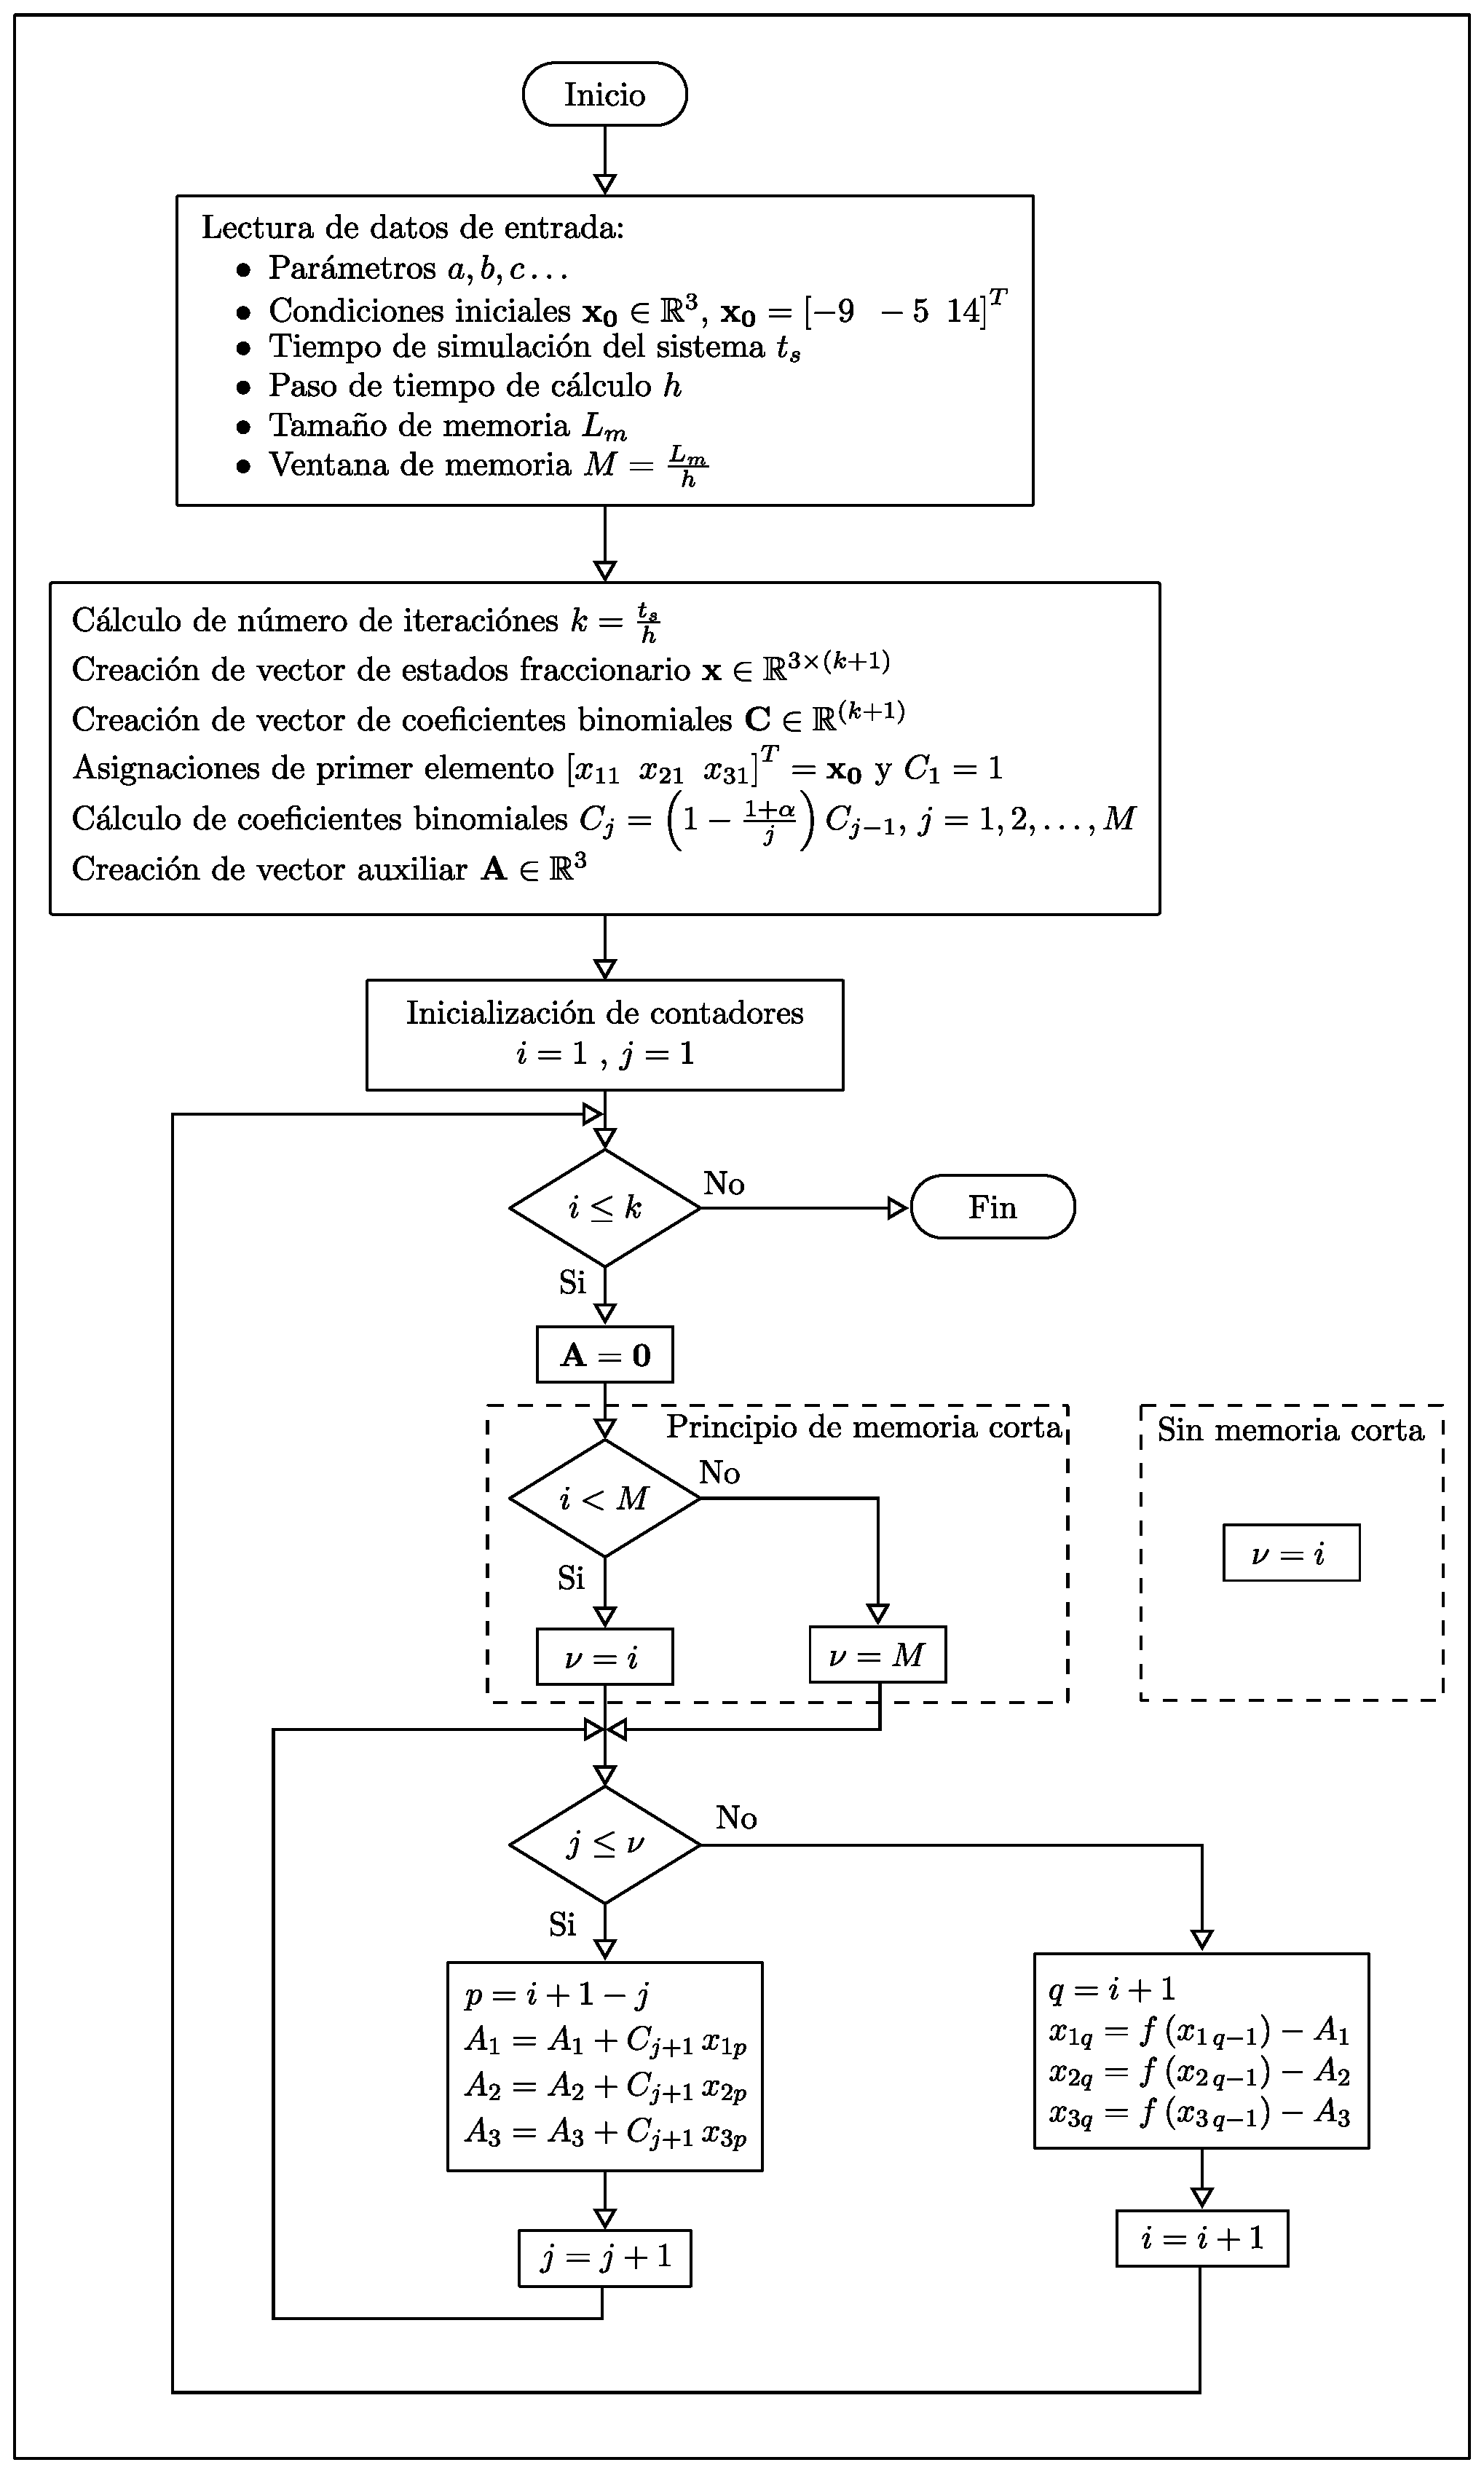
\includegraphics[width=0.6\textwidth]{imagenes/diag_flug_GL.eps}
	\caption{Diagrama de flujo de método numérico de GL.}
	\label{fig:diagrama_flujo}
	\end{figure}
	
	

	\section{Caos}
	
	El caos se refiere a un tipo de comportamiento dinámico complejo que posee algunas características muy especiales, tales como extrema sensibilidad a pequeñas variaciones de la condición inicial, trayectorias encerradas en el espacio de fase con al menos un exponente de Lyapunov positivo y un espectro en potencia continuo.
	
	En otras palabras, el caos es un comportamiento impredecible de un sistema determinista que presenta una sensibilidad muy grande a las condiciones iniciales.
	
	\section{Exponente de Lyapunov}
	
	La principales formas de caracterización de los sistemas caóticos son la dimension fractal, la entropía de Kolmogorov-Sinai y el espectro de Lyapunov. Entre ellos, el exponente de Lyapunov proporciona una forma de determinar si el comportamiento de un sistema es caótico. Los exponentes de Lyapunov dan la descripción  de la presencia de un flujo determinista no periódico, por lo tanto, son una medida asintótica que caracteriza la tasa media de crecimiento (o disminución) de pequeñas
perturbaciones a las soluciones de un sistema dinámico. 

Los exponentes de Lyapunov proporcionan medidas cuantitativas de la sensibilidad de respuesta de un sistema dinámico a pequeños cambios en las condiciones iniciales. El número de exponentes de Lyapunov es igual al numero de variables de estado, y si al menos uno
es positivo, esto es un indicador de caos. Un valor alto del exponente positivo de Lyapunov indica un gran incremento en el grado de impredecibilidad del sistema, por lo tanto, el sistema presenta un comportamiento dinámico más complejo.

\section{Oscilador caótico de múltiples enrollamientos basado en series de funciones saturadas}

	Este oscilador caótico también conocido como SNLF (Funciones No Lineales Saturadas) se describe por las tres ecuaciones diferenciales como se muestra en (\ref{ec:oscilador}), donde $a, b, c$ y $d_{1}$ son constantes positivas que pueden tener valores en el intervalo $[0,1]$. El sistema dinámico esta controlado por una aproximación PWL (Piecewise-linear) que describe la serie de  funciones saturadas  $f$, que se obtiene de la siguiente manera: Sea $f_{0}$ la función saturada descrita por (\ref{ec:f0}) donde $\frac{1}{m}$ es la pendiente del segmento del medio y $m>0$; el radial superior $\{  f_{0}(x_{1},m) = 1 \,\,|\,\, x_{1} > m\}$ y el radial inferior $\{  f_{0}(x_{1},m) = -1 \,\,|\,\, x_{1} < -m\}$ se llaman \textit{mesetas saturadas}, y el segmento $\{  f_{0}(x_{1},m) = \frac{x_{1}}{m} \,\,|\,\, |x_{1}| < -m\}$ entre dos mesetas saturadas se llama \textit{pendiente saturada}.
	
	\begin{equation} 
		\begin{array}{lcl}
		\dot{x_{1}} & = & x_{2} \\
		\dot{x_{2}} & = & x_{3}\\
		\dot{x_{3}} & = & -a x_{1} - b x_{2} -c x_{3} + d_{1} f(x_{1};m)
		\end{array}
		\label{ec:oscilador}
	\end{equation}


\begin{equation} 
	f_{0}(x_{1},m)= \left\{ \begin{array}{lcl}
	1 & \text{ si } & x_{1} > m \\
	\frac{x_{1}}{m}& \text{ si } & |x_{1}| \leq m\\
	-1 & \text{ si } & x_{1} < -m
	\end{array}
	\right.
	\label{ec:f0}
\end{equation}


\begin{equation} 
	f_{h}(x_{1},m,h)= \left\{ \begin{array}{lcl}
	2 & \text{ si } & x_{1} > h + m \\
	\frac{x_{1}-h}{m}& \text{ si } & |x_{1} - h| \leq m\\
	0 & \text{ si } & x_{1} < h-m
	\end{array}
	\right.
		\label{ec:fh}
\end{equation}

\begin{equation} 
	f_{-h}(x_{1},m,-h)= \left\{ \begin{array}{lcl}
	0 & \text{ si } & x_{1} > h + m \\
	\frac{x_{1}-h}{m}& \text{ si } & |x_{1} - h| \leq m\\
	-2 & \text{ si } & x_{1} < h-m
	\end{array}
	\right.
		\label{ec:f-h}
\end{equation}


La serie de funciones saturadas para generar $s$ enrollamientos puede definirse como se muestra en (\ref{ec:general_serie}), para $s > 2$.

\begin{equation}
f(x,m) = \sum_{i=0}^{s-2} f_{2i-s+2}(x,m,2i-s+2)
\label{ec:general_serie}
\end{equation}


\begin{figure}[htp]
	\centering
	\subfigure[]{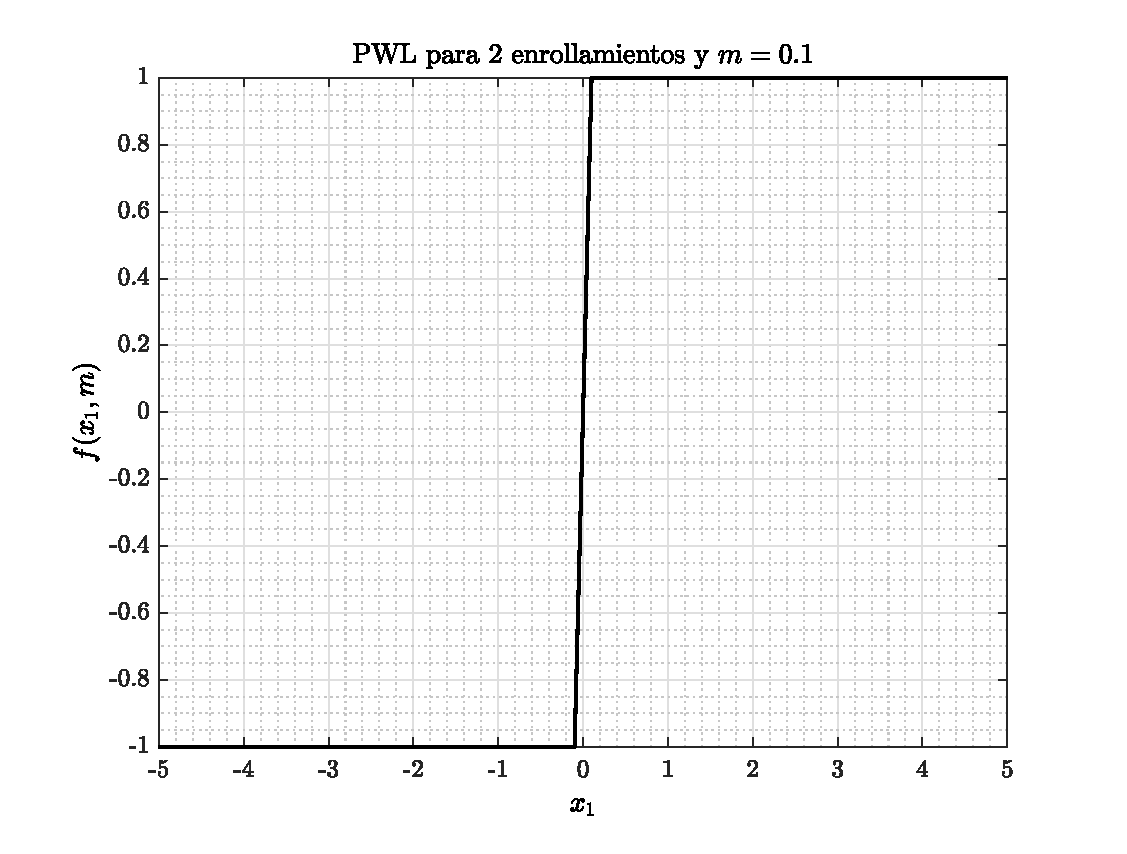
\includegraphics[width=.32\textwidth]{imagenes/enrollamientos2.eps}}
	\subfigure[]{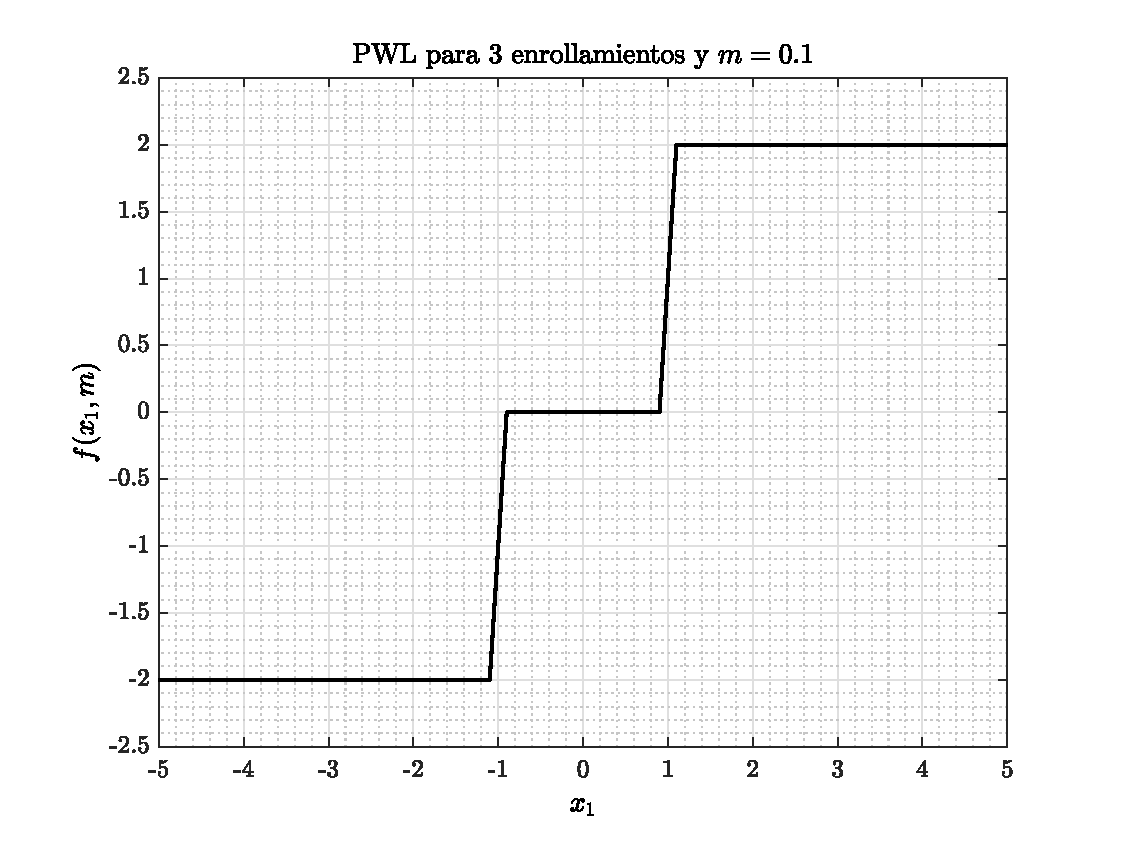
\includegraphics[width=.32\textwidth]{imagenes/enrollamientos3.eps}}
	\subfigure[]{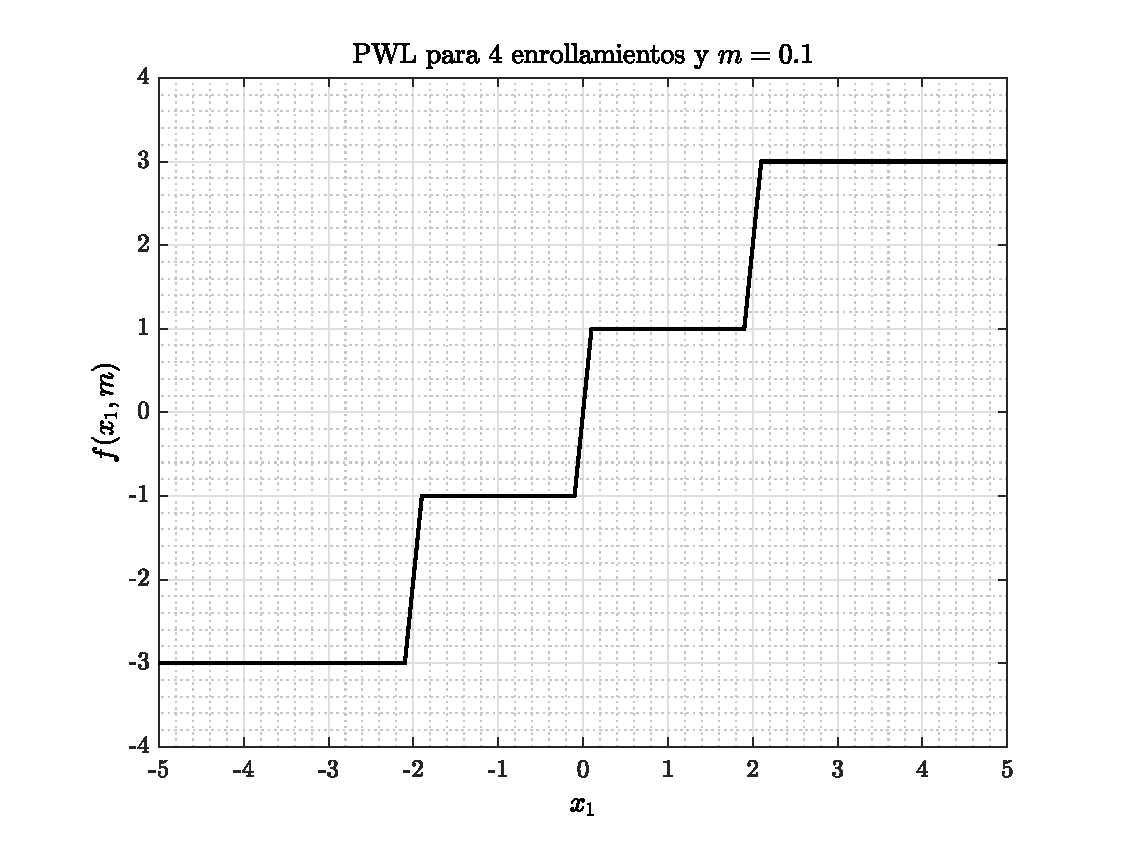
\includegraphics[width=.32\textwidth]{imagenes/enrollamientos4.eps}}
	\caption{Diferentes PWL con $m = 0.1$, (a) 2 enrollamientos, (b) 3 enrollamientos, (c) 4 enrollamientos..}
	\label{fig:pwl}
\end{figure}


\begin{figure}[htp]
	\centering
	\subfigure[]{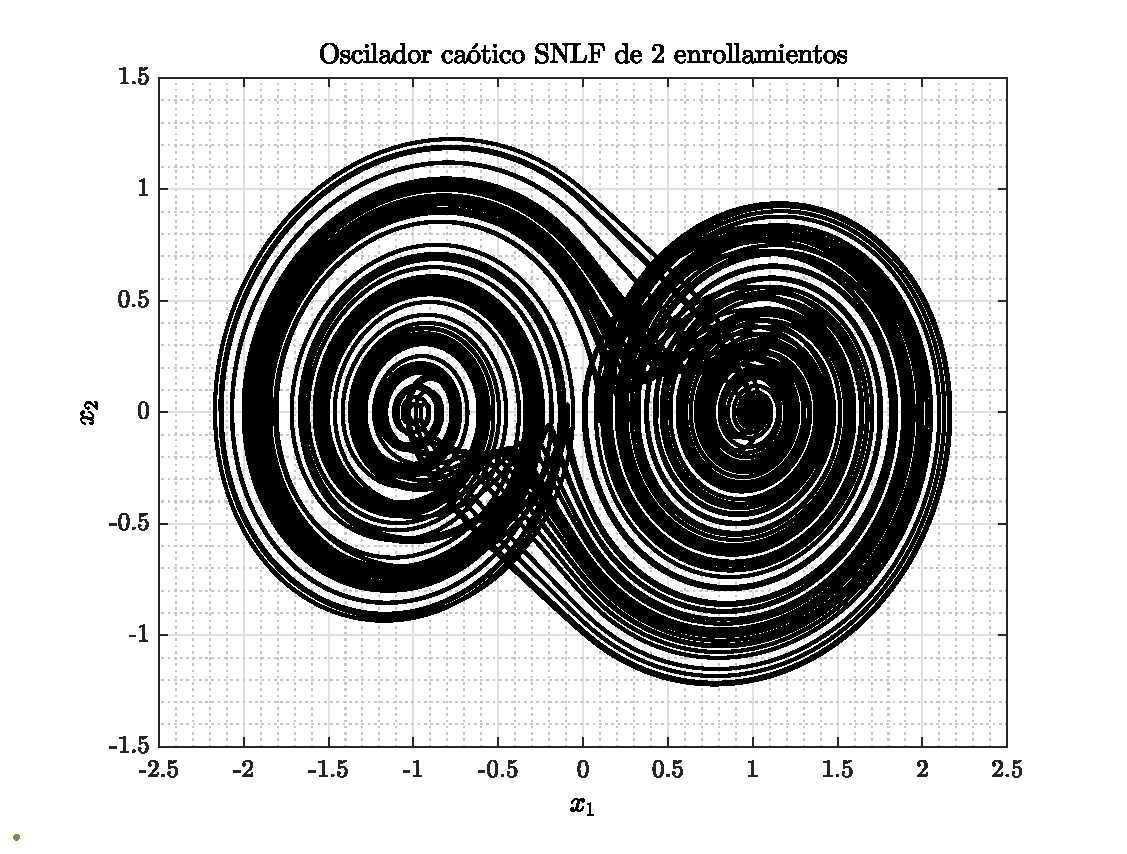
\includegraphics[width=.32\textwidth]{imagenes/osc2.eps}}
	\subfigure[]{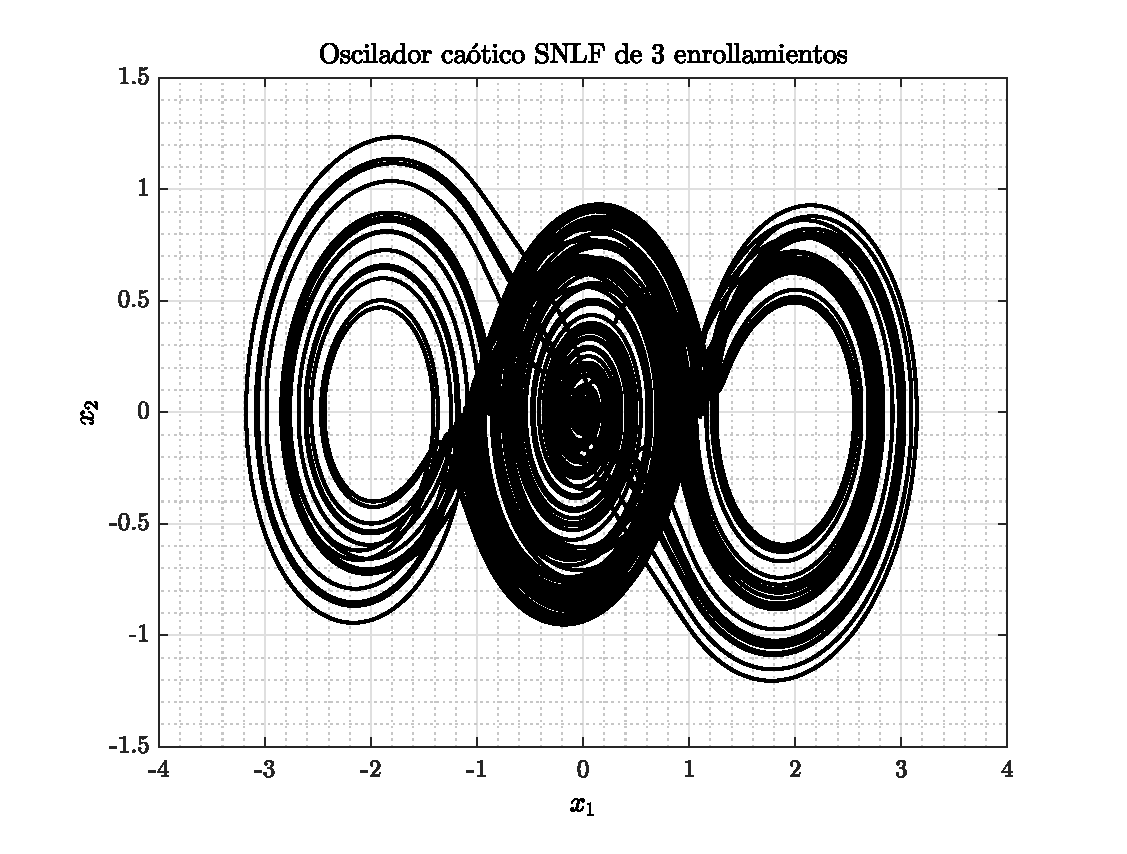
\includegraphics[width=.32\textwidth]{imagenes/osc3.eps}}
	\subfigure[]{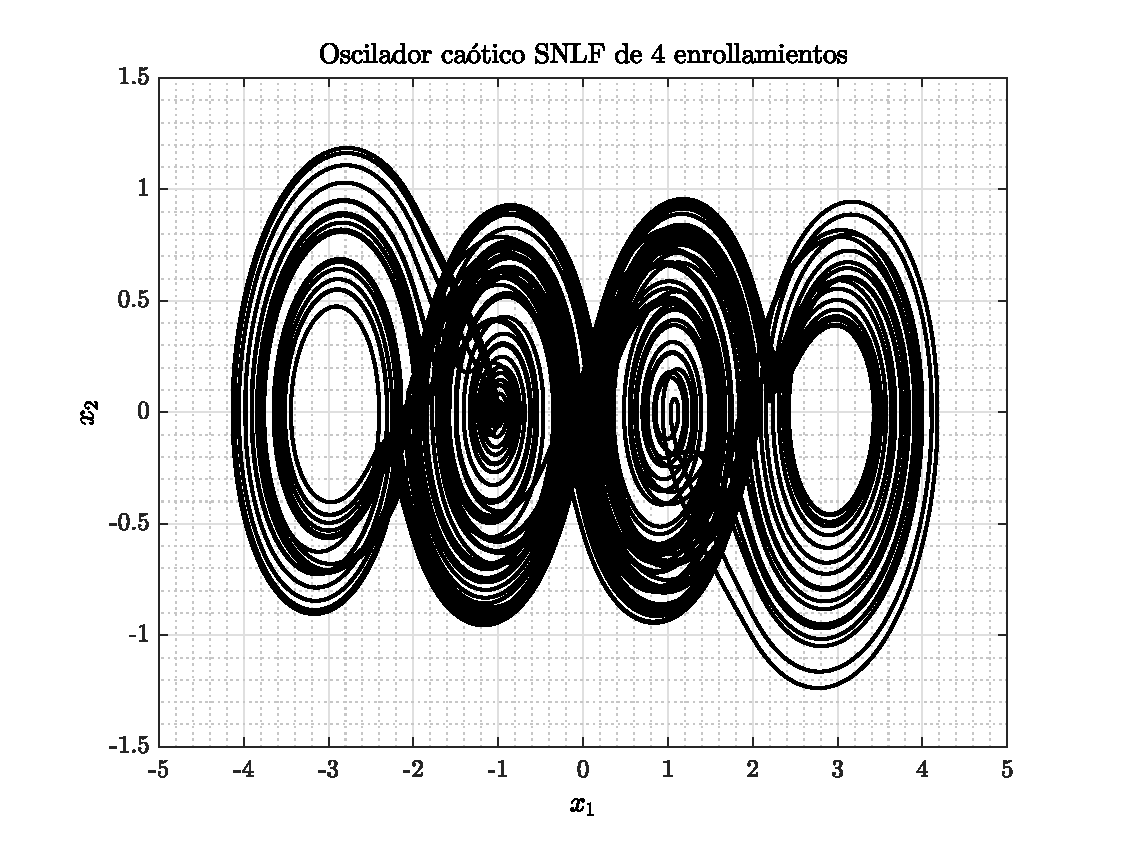
\includegraphics[width=.32\textwidth]{imagenes/osc4.eps}}
	\caption{Osciladores caóticos con $a =b = c = 0.7$ y $\alpha = 1$, (a) 2 enrollamientos, (b) 3 enrollamientos, (c) 4 enrollamientos.}
	\label{fig:osciladores}
\end{figure}


\section{Comprobación de algoritmo con FDE12}

FDE12 resuelve un problema de valor inicial para una ecuación diferencial no lineal de orden faccionario (Fractional Diferential Equation). El código implementa el método predictor-corrector PECE de Adams-Bashforth-Moulton. Para utilizarlo se ocuparon los Códigos \ref{cod:snlf} y \ref{cod:fde12util}.

Para comprobar que nuestro algoritmo numérico de GL funciona se pusieron a prueba tanto GL numérico cono FDE12 y se graficaron sus respuestas para analizar los atractores que generaron, estos tuvieron la misma forma y por ende podemos concluir que el algoritmo funciona correctamente.


\begin{figure}[htp]
	\centering
	\subfigure[]{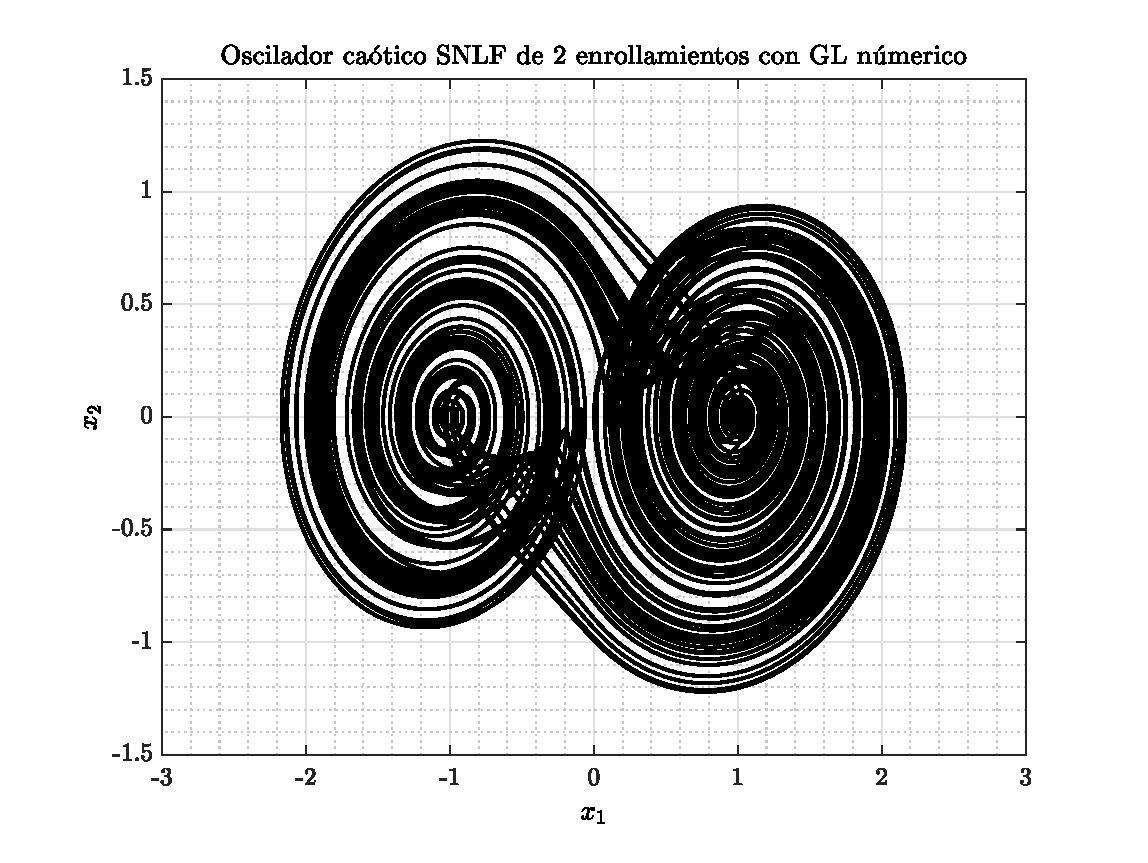
\includegraphics[width=.32\textwidth]{imagenes/gl_num.eps}}\hspace{2cm}
	\subfigure[]{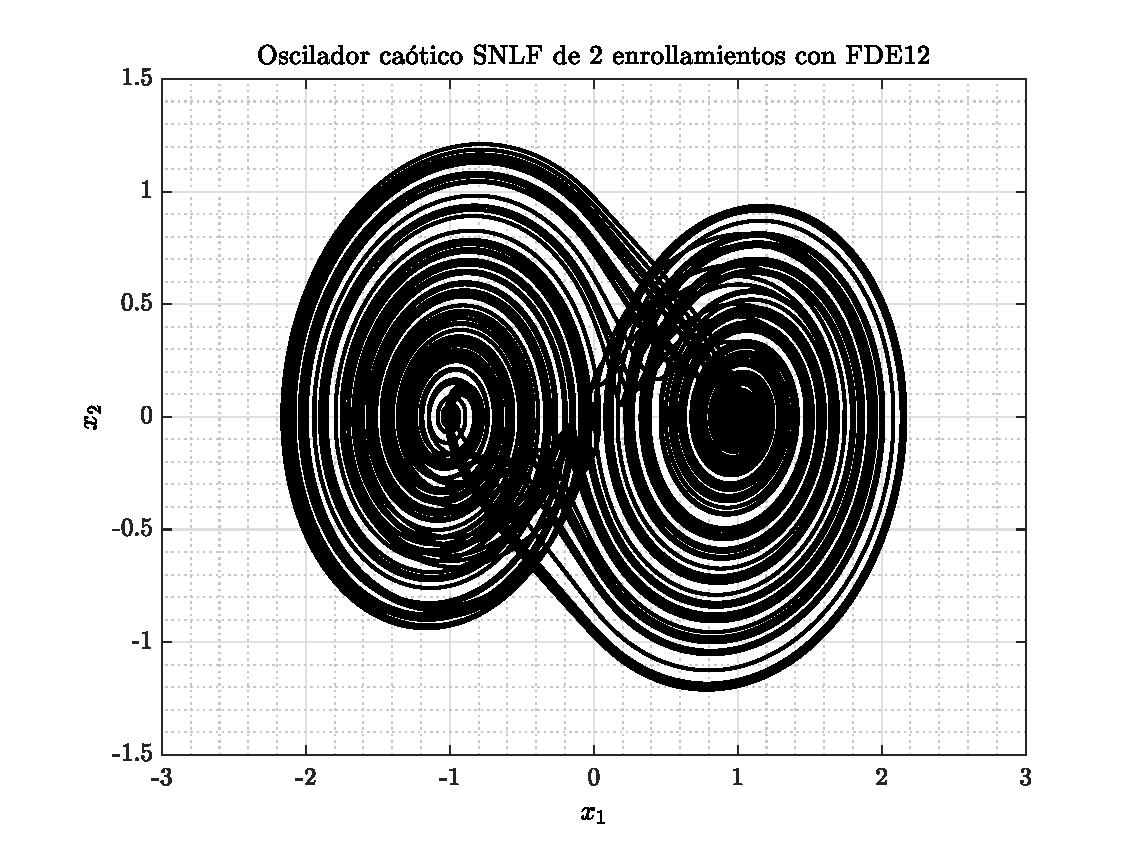
\includegraphics[width=.32\textwidth]{imagenes/fde12_2en.eps}}
	\caption{Osciladores caóticos de 2 enrollamientos con $a =b = c = 0.7$ y $\alpha = 1$, (a) GL numérico, (b) FDE12.}
	\label{fig:glvsfde12}
\end{figure}


\section{TISEAN 3.0.1}

\subsection{¿Qué es?}

TISEAN es un proyecto de software para el análisis de series de tiempo con métodos basados en la teoría de sistemas dinámicos deterministas no lineales, o teoría del caos. Tiene licencia según los términos GPL version 2. Dentro de este software existe la función \textbf{lyap\_{}spec}, la cual estima todo el espectro de exponentes de Lyapunov para una serie de tiempo dada, posiblemente multivariante. Todo el espectro significa: si se dan $d$ componentes y la dimensión de embebida es $m$, se determinarán $m * d$ exponentes. El método se basa en el trabajo de Sano y Sawada.

\subsection{Instalación}
Para instalar TISEAN 3.0.1 se necesitan realizar los siguientes pasos 

\begin{enumerate}
\item Ingresar a: \url{https://www.pks.mpg.de/tisean//Tisean_3.0.1/index.html} buscar \textbf{download page} y descargar el archivo \textbf{TISEAN\_{}3.0.1.tar.gz.}

\item Descomprimirlo utilizando los siguientes comandos: gunzip TISEAN\_{}3.0.1.tar.gz y tar -vxf TISEAN\_{}3.0.1.tar

\item Instalarlo utilizando los pasos descritos en la pagina web.

\end{enumerate}

\subsection{Utilización de lyap\_{}spec}

De todos los parámetros que se pueden modificar en el programa lyap\_{}spec los más importantes a tener en cuenta son:

\begin{enumerate}
	\item \textbf{-x\#} el cual nos permite ignorar las primeras \# lineas del archivo que contenga la serie de tiempo del sistema, de esta manera se saltan los transitorios del sistema y hacemos más rápido el análisis. 
	\item \textbf{-c\#} es el número de columna a leer en el archivo de series de tiempo. Ejemplo -c1 significa leer la primera columna y -c1,2,3 leer las tres columnas, sin embargo este valor se sobrescribe si me modifica el parámetro \textbf{-m\#} .
	\item \textbf{-m\#,\#} es el número de componentes, dimensión embebida. Si solo queremos analizar una variable de estado ocupamos -m1,3, y si queremos utilizar tres variables de estados -m3,1, al modificar este parámetro se eligen automáticamente el número de columnas necesarias a utilizar y se puede prescindir del parámetro -c.
\end{enumerate}

Los demás parámetros los podemos dejar por defecto ya que modificarlos no agrega mucho al cálculo de la dimensión Kaplan-Yorke, por lo tanto para ejecutar lyap\_{}spec se utiliza la siguiente linea de código:

\begin{center}
/.lyap\_{}spec gl\_{}output.txt -x30000 -m3,1 -k100 -oKYout.txt
\end{center}
donde gl\_{}output.txt es la serie de tiempo del método numérico de GL y Xout.txt es el archivo de salida donde se escribirán los resultados de lyap\_{}spec.




\section{Optimización}

Consisten en determinar el valor máximo o mínimo de una función con respecto a una variable o varias variables, encontrando la mejor solución de todas las soluciones posibles. En general el problema se puede definir como:


\[
	\begin{array}{c}
		\text{Minimizar:} \,\, f(\mathbf{x}) \\
		\mathbf{x} \in \Psi \subseteq \mathbb{R}^{n}
	\end{array}
\]

\[
	\begin{array}{c}
		\text{Sujeto a:}  \quad g(\mathbf{x}) \leq 0 \quad \text{y} \quad h(\mathbf{x}) = 0
	\end{array}
\]


		
donde $\mathbf{x} = [x_{1}, x_{2}, \ldots , x_{n}]^{T}$ es un vector que contiene todas las variables de la función, $f(\mathbf{x})$ es llamada función objetivo la cual mide la calidad de la solución y $\Psi$ es el conjunto de puntos que cumplen las restricciones del problema, conocida como zona factible. De mismo modo se pueden agregar restricciones en la forma de desigualdad como $g(\mathbf{x})$ o igualdad como $y(\mathbf{x})$.

Para problemas no lineales, multimodales o de más de tres variables se justifica utilizar heurísticas para la optimización. Si se desea cambiar el problema a maximizar solo es necesario agregar un signo menos a la función objetivo. 


\section{Evolución Diferencial (ED)}
\subsection{Introducción}
La Evolución Diferencial (DE) es un método de búsqueda directa que utiliza $N_{p}$ vectores de parámetros $D$-dimensionales:
\begin{equation}
x_{i,G}, i = 1, 2, \ldots , N_{p}
\end{equation}
como población para cada generación $G$. $N_{p}$ no cambia durante el proceso de minimización. La población del vector inicial se elige al azar y debe cubrir la totalidad del espacio de parámetros. Como regla, asumiremos una distribución de probabilidad uniforme para todas las decisiones aleatorias a menos que se indique lo contrario. La ED genera un nuevos vectores de parámetros sumando la diferencia ponderada entre dos vectores de población a un tercer vector. Dejemos que esta operación se llame \textbf{mutación}. Los parámetros del vector mutado luego se mezclan con los parámetros de otro vector predeterminado, el \textbf{vector objetivo}, para producir el llamado \textbf{vector de prueba}. La mezcla de parámetros a menudo se denomina
\textbf{recombinación} (Crossover). Si el vector de prueba produce un valor de función de costo más bajo que el vector objetivo, el vector de prueba
reemplaza el vector objetivo en la siguiente generación. Esta última operación se llama \textbf{selección}. Cada vector de población tiene que servir una vez como vector objetivo para que $N_{p}$ competiciones tengan lugar en una generación.

\subsection{Mutación}

Por cada vector objetivo $x_{i,G}, i = 1, 2, \ldots , N_{p}$, un vector mutado es generado de acuerdo a:
\begin{equation}
v_{i,G+1} = x_{r_{1},G} + F (x_{r_{2},G} -x_{r_{3},G})
\end{equation}
con indices aleatorios $r_{1}, r_{2}, r_{3} \in \{1,2, \ldots, N_{p}\}$, enteros, mutuamente diferentes y $F> 0$. Los números enteros $r_{1}, r_{2}, r_{3}$ elegidos aleatoriamente también se eligen para ser diferentes del índice de ejecución $i$, de modo que $N_{p}$ debe ser mayor o igual a cuatro para permitir este condición. $F$ es un factor real y constante  $\in [0, 2]$ que controla la amplificación de la variación diferencial $(x_{r_{2},G} -x_{r_{3},G})$.

\subsection{Recombinación}

Para aumentar la diversidad de los vectores de parámetros perturbados, el cruce es introducido. Con este fin, el vector de prueba:
\begin{equation}
u_{i,G+1} = (u_{1i,G+1}, u_{2i,G+1}, \ldots , u_{Di,G+1})
\end{equation}
es formado, donde:

\begin{equation} 
	u_{ji,G+1} = \left\{ \begin{array}{lcl}
	v_{ji,G+1} & \text{ si } & \text{randb}(j) \leq C_{r} \quad \text{o} \quad j = \text{rnbr}(i) \\
	x_{ji,G+1}& \text{ si } &\text{randb}(j) > C_{r} \quad \text{y} \quad j \neq \text{rnbr}(i) \\
	\end{array}
	\right.
	\label{ec:recom}
\end{equation}
con $j = 1,2, \ldots D$, donde $\text{randb}(j)$ es la j-ésima evaluación de un generador de números aleatorios uniforme con resultado $\in [0,1]$. $C_{r}$ es la constante de cruce $\in [0, 1]$ que debe determinarse por el usuario. $\text{rnbr}(i)$ es un índice $\in 1,2, \ldots D$ elegido aleatoriamente que asegura que
$u_{ji,G+1}$ tiene al menos un parámetro de $v_{ji,G+1}$.

\subsection{Comprobación de límites}

Después de realizar la mutación es necesario comprobar que el vector mutado se encuentre dentro de los límites $L_{B}$ (Low Boundary) y $H_{B}$ (High Boundary) de lo contrario es necesario generar una nueva solución aleatoria o redondear al límite más cercano.

\subsection{Selección}

Para decidir si debe convertirse o no en miembro de la generación $G + 1$, el vector de prueba $u_{i,G+1}$ se compara con el vector objetivo $x_{i,G}$ utilizando el criterio codicioso. Si vector $u_{i,G+1}$ produce un valor de función de costo menor que  $x_{i,G}$ entonces  $x_{i,G+1}$ se establece en
$u_{i,G+1}$  de lo contrario, se conserva el antiguo valor $x_{i,G}$.

En el siguiente pseudocódigo se muestra cómo funciona la heurística de ED.

\begin{algorithm}
\caption{Pseudocódigo ED}
\begin{algorithmic}[1]
\REQUIRE Función objetivo, $D$, $N_{p}$, $G$, $F$, $C_{r}$, $L_{B}$, $H_{B}$ 
\STATE Inicializar la población aleatoria ($P$)
\STATE Evaluar función objetivo ($f$) de ($P$)
\FOR{$j = 1$ a $G$ }
	\FOR{$i = 1$ a $N_{p}$ }
		\STATE Generar el vector donador $v$ usando la \textbf{mutación}
		\STATE Realizar la \textbf{recombinación} para generar el vector $u$
	\ENDFOR
	\FOR{$i = 1$ a $N_{p}$ }
		\STATE Comprobar limites de $u$
		\STATE Evaluar la función objetivo ($f_{u}$) para $u$ 
		\STATE Realizar la \textbf{selección} usando $f_{u}$ y $f$ para actualizar $P$
	\ENDFOR
\ENDFOR
\end{algorithmic}
\end{algorithm}




%Esta meta-heuristica depende de dos operadores, de la mutación y de la recombinación.
%
%1997 Storn, Kennegth Price
%Differential Evolution - A simple and efficient heuristic for global optimization over continuous spaces
%
%TLBO, PSO y DE son las metaheuristicas más utilizadas
%Poblacion estocastica
%
%cada solucion es conocida como genome / chromosome 
%cada cromosoma experimenta una mutación seguida de recombinacion
%
%el target vector es la solucion
%target vector $\to$ mutacion  $\to$ Donor vector $\to$ recombination $\to$ trial vector
%
%donor vector $V$ chromosome $X_{i}$ is created as
%
%$F$ scaling factor constant vetween 0 and 2
%$r_{1},r_{2},r_{3} \in \{ 1,2,3, ... N_{p}\}$ Random solutions, y $r_{1} \neq r_{2} \neq r_{3} \neq i$
%
%Target vector no se involca en la mutacion
%
%Un total de 4 vectores se invoca en la mutacion del target vector y por lo tanto $N_{p} \geq 4$
%
%\begin{equation}
%V = X_{r_1} + F(X_{r_2} - X_{r_3})
%\end{equation}
%
%Ahora se aplica la recombinación binomial (uniforme) para todas las variables del sistema
%
%\begin{equation} 
%	u^{j} = \left\{ \begin{array}{lcl}
%	v^{j} & \text{ si } & r \leq p_{c} \quad \text{o} \quad j = \delta \\
%	x^{j}& \text{ si } & r > p_{c} \quad \text{y} \quad j \neq \delta \\
%	\end{array}
%	\right.
%	\label{ec:recom}
%\end{equation}
%
%$p_{c}$ crossover probability
%
%$\delta$ randomly selected variable location $\delta \in \{ 1,2,3 \ldots D\}$
%
%$r$ random number betwen 0 and 1
%
%$u^{j}$  $j^{\text{th}}$ variable of trial vector
%
%$v^{j}$  $j^{\text{th}}$ variable of donor vector
%
%$x^{j}$ $ j^{\text{th}}$ variable of target vector


\section{Problemas de prueba para optimización}
	\subsection{Función esfera}
	\begin{equation}
		f(\mathbf{x}) = \sum_{i=1} ^{d} x_{i}^{2}
	\end{equation}
	\textbf{Descripción:} Dimensión: $d$. La función esfera tiene $d$ mínimos locales excepto por el global. Es continua, convexa y unimodal.
	
	\textbf{Dominio de entrada:} La función ese evaluá normalmente en el hipercubo  $x_{i} \in [-5.12, 5.12]$, para toda $i = 1, \ldots, d$.
	
	\textbf{Mínimo global:} $f(\mathbf{x^{*}}) = 0$, en $\mathbf{x^{*}} = (0, \ldots , 0)$.
	
	
	\subsection{Función Rosenbrock}
	\begin{equation}
		f(\mathbf{x}) = \sum_{i=1} ^{d-1} \left[  100(x_{i+1} - x_{i}^{2})^{2} + (x_{i} -1)^{2}  \right]
	\end{equation}
	
	\textbf{Descripción:} 
	Dimensión: $d$.	La función Rosenbrock, también conocida como función Valley o Banana, es un problema de prueba popular para los algoritmos de optimización basados en gradientes. La función es unimodal y el mínimo global se encuentra en un valle parabólico estrecho. Sin embargo, aunque este valle es fácil de encontrar, la convergencia al mínimo es difícil.
	
	\textbf{Dominio de entrada:} La función ese evaluá normalmente en el hipercubo  $x_{i} \in [-5, 10]$, para toda $i = 1, \ldots, d$, aunque puede estar restringida en el hipercubo  $x_{i} \in [-2.048, 2.048]$, para toda $i = 1, \ldots, d$.
	
	\textbf{Mínimo global:} $f(\mathbf{x^{*}}) = 0$, en $\mathbf{x^{*}} = (1, \ldots , 1)$.


\section{Prueba de heuristica ED}

Para asegurarnos que nuestra heurística esta funcionando correctamente utilizamos la función esfera y la función Rosenbrock para 10 variables. La heurística esta escrita en python3 y utilizando los parámetros de las Figuras (a) de \ref{fig:tabs_rosen} y \ref{fig:tabs_esfera} se obtuvieron los resultados de las Figuras (b) de \ref{fig:tabs_rosen} y \ref{fig:tabs_esfera}.

	
\begin{figure}[htp]
	\centering
	\subfigure[]{
		\begin{tabular}{ccc}
			\hline                                             
			Parámetro & Nombre &Valor \\                     
			\hline 
			$D$ & Dimensión & 10\\                                            
			$N_{p}$ & Población & 60\\                                            
			$F$ & Constante de diferenciación & 0.9\\
			$C_{r}$ & Constante de cruza & 0.5\\
			$G$ & Número de generaciones & 5000\\
			$L$ & Límite inferior & -5.12\\
			$H$ & Límite Superior & 5.12\\
			\hline                                             
		\end{tabular}  	                                   
	}\hspace{2cm}
	\subfigure[]{
		\begin{tabular}{cc}
			\hline                                             
			$x_{i}$ & Valor \\                     
			\hline                                           
			$1$ & -3.1582697774443324e-45\\
			$2$ & 3.342055372731574e-44\\
			$3$ & 2.0277780119756814e-44\\
			$4$ & -6.544736342264586e-44\\
			$5$ & 2.66093268020275e-44\\
			$6$ & -8.976013629979016e-46\\
			$7$ & -1.4290248717362062e-44\\
			$8$ & 5.275161620435796e-44\\
			$9$ & 1.4464108120607483e-44\\
			$10$ & 1.766707533599044e-44\\
			$f(\mathbf{x})$ & 1.0038595981280693e-86\\
			\hline                                             
		\end{tabular}
	}
	\caption{(a) Tabla de parámetros para heurística ED de función esfera. (b) Tabla de resultados de ED para función esfera.}
	\label{fig:tabs_esfera}
\end{figure}

\begin{figure}[htp]
	\centering
	\subfigure[]{
		\begin{tabular}{ccc}
			\hline                                             
			Parámetro & Nombre &Valor \\                     
			\hline 
			$D$ & Dimensión & 10\\                                            
			$N_{p}$ & Población & 60\\                                            
			$F$ & Constante de diferenciación & 0.9\\
			$C_{r}$ & Constante de cruza & 0.5\\
			$G$ & Número de generaciones & 5000\\
			$L$ & Límite inferior & -2.048\\
			$H$ & Límite Superior & 2.048\\
			\hline                                             
		\end{tabular}  	                                   
	}\hspace{2cm}
	\subfigure[]{
		\begin{tabular}{cc}
			\hline                                             
			$x_{i}$ & Valor \\                     
			\hline                                           
			$1$ & 0.9999703704219989\\
			$2$ & 0.9999001982008784\\
			$3$ & 0.9999754920845646\\
			$4$ & 0.9999905572609116\\
			$5$ & 1.000042007011715\\
			$6$ & 1.000145028356835\\
			$7$ & 1.0002166650657043\\
			$8$ & 1.000294147734143\\
			$9$ & 1.0004887885050615\\
			$10$ & 1.0010586554627545\\
			$f(\mathbf{x})$ & 8.659037967753027e-06\\
			\hline                                             
		\end{tabular}
	}
	\caption{(a) Tabla de parámetros para heurística ED de función Rosenbrock. (b) Tabla de resultados de ED para función Rosenbrock.}
	\label{fig:tabs_rosen}
\end{figure}


Si comparamos los resultados de la heurística con los teóricos podemos percatarnos inmediatamente que funciona a la perfección y podemos utilizarla con seguridad, sin embargo es importante resaltar que la heurística podría mejorar si se modifican los parámetros.




\section{Optimización de los parámetros del oscilador caótico SNLF}

\subsection{Función objetivo para oscilador SNLF}

\textbf{Descripción:} 
	Dimensión: $d = 4$.	La función objetivo es el programa \textbf{lyap\_{}spec} cuya salida es la dimensión Kaplan-York del sistema y cuya entrada es la serie de tiempo generada por el programa \textbf{gl.c}.
	
	\textbf{Dominio de entrada:} El programa \textbf{gl.c} genera la serie de tiempo del sistema caótico utilizando el método numérico de GL y sus entradas son  $a, b, c, d \in [0.01, 1]$, para toda $a,b,c,d$.
	
	\textbf{Maximizar:} El objetivo de aplicar la heurística es maximizar la Kaplan-York del sistema y por ende es necesario agregar un signo menos a la salida de la dimensión Kaplan-York.
	
\subsection{Restricciones}
\begin{enumerate}
	\item Si la serie de tiempo tiende al infinito el programa lyap\_{}spec falla y la heurística deja de funcionar, por lo tanto se añade la restricción que las series de tiempo estén dentro del rango de $[-50,50]$ para asegurarnos que lyap\_{}spec funcione correctamente.
	\item Si la serie converge a un solo valor no vale la pena generar la serie de tiempo por el programa lyap\_{}spec .
	\item Calcular la serie de tiempo toma aproximadamente 5 seg, y calcular la dimensión Kaplan-York toma 10 seg. Por lo tanto es necesario elegir con cuidado la población y el número de generaciones.
\end{enumerate}

Como referencia se sabe de la literatura que el oscilador SNLF para los valores $x_{1} = x_{2} = x_{3} = x_{4} = 0.7$ se obtiene KY$=2.003263$.

\subsection{Restructuración de pseudocódigo}

Se necesitaron los siguientes modificaciones al pseudocódigo para que la heurística funcionara correctamente.

\begin{algorithm}
\caption{Pseudocódigo ED}
\begin{algorithmic}[1]
\REQUIRE Función objetivo, $D$, $N_{p}$, $G$, $F$, $C_{r}$, $L_{B}$, $H_{B}$ 
\WHILE{Población no este llena}
	\STATE Inicializar la población aleatoria ($P$)
	\STATE Comprobar restricciones 
\ENDWHILE
\STATE Evaluar función objetivo ($f$) de ($P$)
\FOR{$j = 1$ a $G$ }
	\FOR{$i = 1$ a $N_{p}$ }
		\WHILE{Vector donador no sea valido}
			\STATE Generar el vector donador $v$ usando la \textbf{mutación}
			\STATE Comprobar restricciones 
		\ENDWHILE
	\STATE Realizar la \textbf{recombinación} para generar el vector $u$
	\ENDFOR
	\FOR{$i = 1$ a $N_{p}$ }
		\STATE Comprobar limites de $u$
		\STATE Evaluar la función objetivo ($f_{u}$) para $u$ 
		\STATE Realizar la \textbf{selección} usando $f_{u}$ y $f$ para actualizar $P$
	\ENDFOR
\ENDFOR
\end{algorithmic}
\end{algorithm}


\subsection{Utilización de la heurística}

\subsubsection{Resultados de prueba 1}
Para esta prueba se utilizaron los parámetros mostrados en Tabla (a) de la Figura \ref{fig:tabs_res1}, se obtuvieron los resultados de la Tabla (b) de la misma Figura. y el oscilador resultante se muestra en la Figura \ref{fig:res1}.
\begin{figure}[htp]
	\centering
	\subfigure[]{
		\begin{tabular}{ccc}
			\hline                                             
			Parámetro & Nombre &Valor \\                     
			\hline 
			$D$ & Dimensión & 4\\                                            
			$N_{p}$ & Población & 10\\                                            
			$F$ & Constante de diferenciación & 0.9\\
			$C_{r}$ & Constante de cruza & 0.5\\
			$G$ & Número de generaciones & 10\\
			$L$ & Límite inferior & 0.01\\
			$H$ & Límite Superior & 1.0\\
			\hline                                             
		\end{tabular}  	                                   
	}\hspace{2cm}
	\subfigure[]{
		\begin{tabular}{cc}
			\hline                                             
			$x_{i}$ & Valor \\                     
			\hline                                           
			$1$ & 0.11239836608526878\\
			$2$ & 0.7062035586495738\\
			$3$ & 0.01742061370410969\\
			$4$ & 0.16324569243104947\\
			$f(\mathbf{x})$ & 2.782829\\
			\hline                                             
		\end{tabular}
	}
	\caption{(a) Tabla de parámetros para heurística ED de oscilador SNLF. (b) Tabla de resultados de ED paraoscilador SNLF.}
	\label{fig:tabs_res1}
\end{figure}

\begin{figure}[htp]
	\centering
	\includegraphics[width=.5\textwidth]{imagenes/super1.pdf}
	\caption{Oscilador SNLF con KY$ = 2.782829$.}
	\label{fig:res1}
\end{figure}



\subsubsection{Resultados de prueba 2}
Para esta prueba se utilizaron los parámetros mostrados en Tabla (a) de la Figura \ref{fig:tabs_res2}, se obtuvieron los resultados de la Tabla (b) de la misma Figura. y el oscilador resultante se muestra en la Figura \ref{fig:res2}.
\begin{figure}[htp]
	\centering
	\subfigure[]{
		\begin{tabular}{ccc}
			\hline                                             
			Parámetro & Nombre &Valor \\                     
			\hline 
			$D$ & Dimensión & 4\\                                            
			$N_{p}$ & Población & 10\\                                            
			$F$ & Constante de diferenciación & 0.9\\
			$C_{r}$ & Constante de cruza & 0.5\\
			$G$ & Número de generaciones & 10\\
			$L$ & Límite inferior & 0.01\\
			$H$ & Límite Superior & 1.0\\
			\hline                                             
		\end{tabular}  	                                   
	}\hspace{2cm}
	\subfigure[]{
		\begin{tabular}{cc}
			\hline                                             
			$x_{i}$ & Valor \\                     
			\hline                                           
			$1$ & 0.3337747516106829\\
			$2$ & 0.9744419522364808\\
			$3$ & 0.09963819929121229\\
			$4$ & 0.6296137310167467\\
			$f(\mathbf{x})$ & 2.510171\\
			\hline                                             
		\end{tabular}
	}
	\caption{(a) Tabla de parámetros para heurística ED de oscilador SNLF. (b) Tabla de resultados de ED paraoscilador SNLF.}
	\label{fig:tabs_res2}
\end{figure}

\begin{figure}[htp]
	\centering
	\includegraphics[width=.5\textwidth]{imagenes/super2.pdf}
	\caption{Oscilador SNLF con KY$ = 2.510171$.}
	\label{fig:res2}
\end{figure}



\subsubsection{Resultados de prueba 3}
Para esta prueba se utilizaron los parámetros mostrados en Tabla (a) de la Figura \ref{fig:tabs_res3}, se obtuvieron los resultados de la Tabla (b) de la misma Figura. y el oscilador resultante se muestra en la Figura \ref{fig:res3}.
\begin{figure}[htp]
	\centering
	\subfigure[]{
		\begin{tabular}{ccc}
			\hline                                             
			Parámetro & Nombre &Valor \\                     
			\hline 
			$D$ & Dimensión & 4\\                                            
			$N_{p}$ & Población & 10\\                                            
			$F$ & Constante de diferenciación & 0.9\\
			$C_{r}$ & Constante de cruza & 0.5\\
			$G$ & Número de generaciones & 10\\
			$L$ & Límite inferior & 0.01\\
			$H$ & Límite Superior & 1.0\\
			\hline                                             
		\end{tabular}  	                                   
	}\hspace{2cm}
	\subfigure[]{
		\begin{tabular}{cc}
			\hline                                             
			$x_{i}$ & Valor \\                     
			\hline                                           
			$1$ & 0.3337747516106829\\
			$2$ & 0.8336214768080837\\
			$3$ & 0.21575244523693599\\
			$4$ & 0.5082457095833637\\
			$f(\mathbf{x})$ & 2.318272\\
			\hline                                             
		\end{tabular}
	}
	\caption{(a) Tabla de parámetros para heurística ED de oscilador SNLF. (b) Tabla de resultados de ED paraoscilador SNLF.}
	\label{fig:tabs_res3}
\end{figure}

\begin{figure}[htp]
	\centering
	\includegraphics[width=.5\textwidth]{imagenes/super3.pdf}
	\caption{Oscilador SNLF con KY$ = 2.318272$.}
	\label{fig:res3}
\end{figure}


\subsubsection{Resultados de prueba 4}
Para esta prueba se utilizaron los parámetros mostrados en Tabla (a) de la Figura \ref{fig:tabs_res4}, se obtuvieron los resultados de la Tabla (b) de la misma Figura. y el oscilador resultante se muestra en la Figura \ref{fig:res4}.
\begin{figure}[htp]
	\centering
	\subfigure[]{
		\begin{tabular}{ccc}
			\hline                                             
			Parámetro & Nombre &Valor \\                     
			\hline 
			$D$ & Dimensión & 4\\                                            
			$N_{p}$ & Población & 10\\                                            
			$F$ & Constante de diferenciación & 0.9\\
			$C_{r}$ & Constante de cruza & 0.5\\
			$G$ & Número de generaciones & 10\\
			$L$ & Límite inferior & 0.01\\
			$H$ & Límite Superior & 1.0\\
			\hline                                             
		\end{tabular}  	                                   
	}\hspace{2cm}
	\subfigure[]{
		\begin{tabular}{cc}
			\hline                                             
			$x_{i}$ & Valor \\                     
			\hline                                           
			$1$ & 0.1289450809800962\\
			$2$ & 0.7423872806486553\\
			$3$ & 0.09270994812182803\\
			$4$ & 0.5935300678553914\\
			$f(\mathbf{x})$ & 2.510171\\
			\hline                                             
		\end{tabular}
	}
	\caption{(a) Tabla de parámetros para heurística ED de oscilador SNLF. (b) Tabla de resultados de ED paraoscilador SNLF.}
	\label{fig:tabs_res4}
\end{figure}


\begin{figure}[htp]
	\centering
	\includegraphics[width=.5\textwidth]{imagenes/super4.pdf}
	\caption{Oscilador SNLF con KY$ = 2.861136$.}
	\label{fig:res4}
\end{figure}


\newpage
\section{Códigos}
\label{sec:codigos}

\lstinputlisting[style = MATLAB, caption =  Función de series saturadas., label = cod:sat]{codigos/sat_fun_k.m}
\lstinputlisting[style = MATLAB, caption =  Método numérico de GL., label = cod:GL_num]{codigos/gl.m}
\lstinputlisting[style = MATLAB, caption =  Descripción de ecuación diferencial SNLF., label = cod:snlf]{codigos/SNLF.m}
\lstinputlisting[style = MATLAB, caption =  Utilización de FDE12.m., label = cod:fde12util]{codigos/fde12_oscilador.m}


%https://www.math-linux.com/latex-26/faq/latex-faq/article/how-to-write-algorithm-and-pseudocode-in-latex-usepackage-algorithm-usepackage-algorithmic

\bibliographystyle{ieeetr}
\bibliography{bibliografia}

\end{document}